\section{序論}
\subsection{はじめに}
低温で物質が超伝導を示すことは1911年にオランダのH. K. Onnesにより水銀で発見された。のちにこの現象は多くの物質に普遍的であることが分かり、すでに数千種類の超伝導体が発見されている。超伝導状態にある物質は電磁気学的および熱力学的に特徴的な振る舞いを見せる。もっとも典型的な性質は電気抵抗が0となることであり、散逸のない電流ケーブルや高強度の電磁石に応用されている。また磁場に対する応答も、完全に磁場を遮蔽するMeisner効果が一部の金属で現れるなど、金属状態の磁性と劇的に異なる。さらに超伝導体同士を弱く結合すると、巨視的な位相に依存して、Josephson電流と呼ばれる超伝導状態に特有な電流も観測できる。この効果は高感度な磁気センサなどに用いられる。さらに超伝導状態の金属と通常の金属の間の転移の際に比熱に飛びが現れるなど、熱的な振る舞いにも特徴がある。これらの特徴的な物理特性と応用の多彩さから、100年以上に渡り超伝導物理学は物理学の中心的なテーマであり続けてきた。

超伝導物理学の歴史で特に重要なのは、J. G. BednorzとK. A. M\"ullerによる銅酸化物超伝導体の発見である\cite{Bednorz}。
銅酸化物超伝導体は母物質の元素置換により超伝導を発現する\cite{Lee2006}。銅酸化物超伝導体の発見に触発されて多くの人々が元素置換による超伝導物質の探索を行い、液体窒素温度で実現する高温超伝導体\cite{Wu}や、超伝導転移温度$\rm T_c=26K$の鉄系超伝導体\cite{Kamihara}などの異なった物質群も次々に発見された。これらは、いわば化学的な超伝導へのアプローチの成果であって、一部が応用に進展し、さらに銅酸化物超伝導体を内包する強相関電子系物質と金属-絶縁体転移などの研究も刺激した\cite{Lee2006,Imada}。

一方で単純な化学的アプローチは、高温での作成や制御性に難点がある。狙いの組成で母物質に元素を固溶させるのが難しかったり、外部からの刺激で超伝導性を制御できない。そのため異なった手法も近年盛んに研究され、例えば電界(イオンゲート)効果\cite{Ueno,Ueno2,Ye2009}や薄膜効果\cite{Chiang1900}、非平衡過程\cite{Fausti,Hunt2015,Mitrano2016,oike}を用いた手法などが実現されている。これらの効果を用いると、超伝導体以外の物質を超伝導体にスイッチしたり、物質固有の超伝導転移温度$T_c$を制御することができる。

筆者らの研究グループは特に非平衡過程を用いた制御に着目した。後述するように非平衡過程を用いた制御は可逆的であり、また光を用いた制御が可能なのでリソグラフィ技術を用いてパターニングできる。さらにこの手法には新超伝導物質発見の可能性がある。しかし非平衡による超伝導を研究された物質の例は少なく、いまだ応用と理論的な理解は限定されている。

そこで本研究は新規物質としてスズを用い、非平衡過程を経由した超伝導体制御を実証することを目指した。スズは286.4Kより高温で正方晶の金属相(βスズ)が安定である。一方286.4Kより低温において立方晶の半導体相(αスズ)が安定だが、βスズを十分に早く冷却すると構造相転移できずβスズも準安定となる。このβスズを臨界温度3.7K以下に保つと超伝導が現れる。したがって冷却速度(温度履歴)をコントロールすれば、原理的に超伝導体と半導体間の制御・変換が可能である。

αスズとβスズの特性は大きく異なる。αスズは低温で指数関数的に電気抵抗が大きくなるが、超伝導βスズは抵抗で抵抗がゼロとなる。また光学的な性質も異なる。αスズはエネルギー0.018eV(4.4THz)以下の光を透過するが、βスズは反射する。これらの性質から、半導体中の超伝導回路のパターニングは低損失な電気回路のみならず、プラズモニック回路や量子コンピュータなどに有用である。特にスズは地球上に豊富に存在する元素であり、融点が低く取り扱いやすく、また人体への毒性もない。応用の幅広さと取り扱いの簡単さから、本研究にスズは最適であると筆者は考える。

\subsection{元素置換による銅酸化物超伝導体の化学的制御}
銅酸化物超伝導体はMott絶縁体の元素置換により超伝導を発現する\cite{Lee2006}。Mott絶縁体の振る舞いは独立電子近似を超え、物質の電子間の相互作用の効果を考慮に入れないと説明できない。この節ではMott絶縁体の物理に関して概説し、銅酸化物超伝導体について述べる。

孤立した原子核に束縛された電子は離散的なエネルギー準位をとる。しかし原子同士を近づけてゆくと、電子の波動関数は重なり電子同士の相互作用の影響が現れる。多くの場合は相互作用の影響をイオンのポテンシャルに取り入れて、あたかも電子が独立に振る舞うかのように扱う近似が妥当である(独立電子近似)\cite{ashcroft1976}。この近似のもとで、原子間距離が小さくなると電子の重なり積分に比例となる。図\ref{fig:band}にの原子間距離とエネルギー準位の関係を模式的に示す。原子間距離が小さくなると電子のエネルギー順位は幅を持つことが読み取れる。そして結晶構造において多数個の原子が周期的に配列するとき、固体中の電子準位は幅のあるバンド(帯)構造をとる。

このバンド準位をどのように電子が占有するかだけの情報から固体の多くの性質を説明したのが、(狭い意味での)固体のバンド理論である。固体のバンド理論は多くの金属と半導体、絶縁体の性質を説明する。電子がイオンと電荷の中性条件を満たすようにバンド準位を独立に占めていったとき、占有された最大のエネルギー準位の直上に空いた準位があれば、物質は金属となる。一方占有された最大のエネルギー準位の直上に準位が存在しないとき、物質は絶縁体もしくは半導体となる。

Mott絶縁体も通常の絶縁体と同様に、占有された最大のエネルギー準位の直上に準位が存在しないとする描像で理解できる。しかしバンド理論とはバンドの形成のされ方が異なる。この意味で単純なバンド理論ではないが、バンド理論の拡張と言うことができる。一方、現れる量子ホール効果の研究はエネルギー準位の情報だけではなく、エネルギー固有状態の情報(Berry曲率)も必要となるため、バンド理論の枠組みを超えている。
\begin{figure}[!h]
 \begin{minipage}{0.5\hsize}
    \begin{center}
   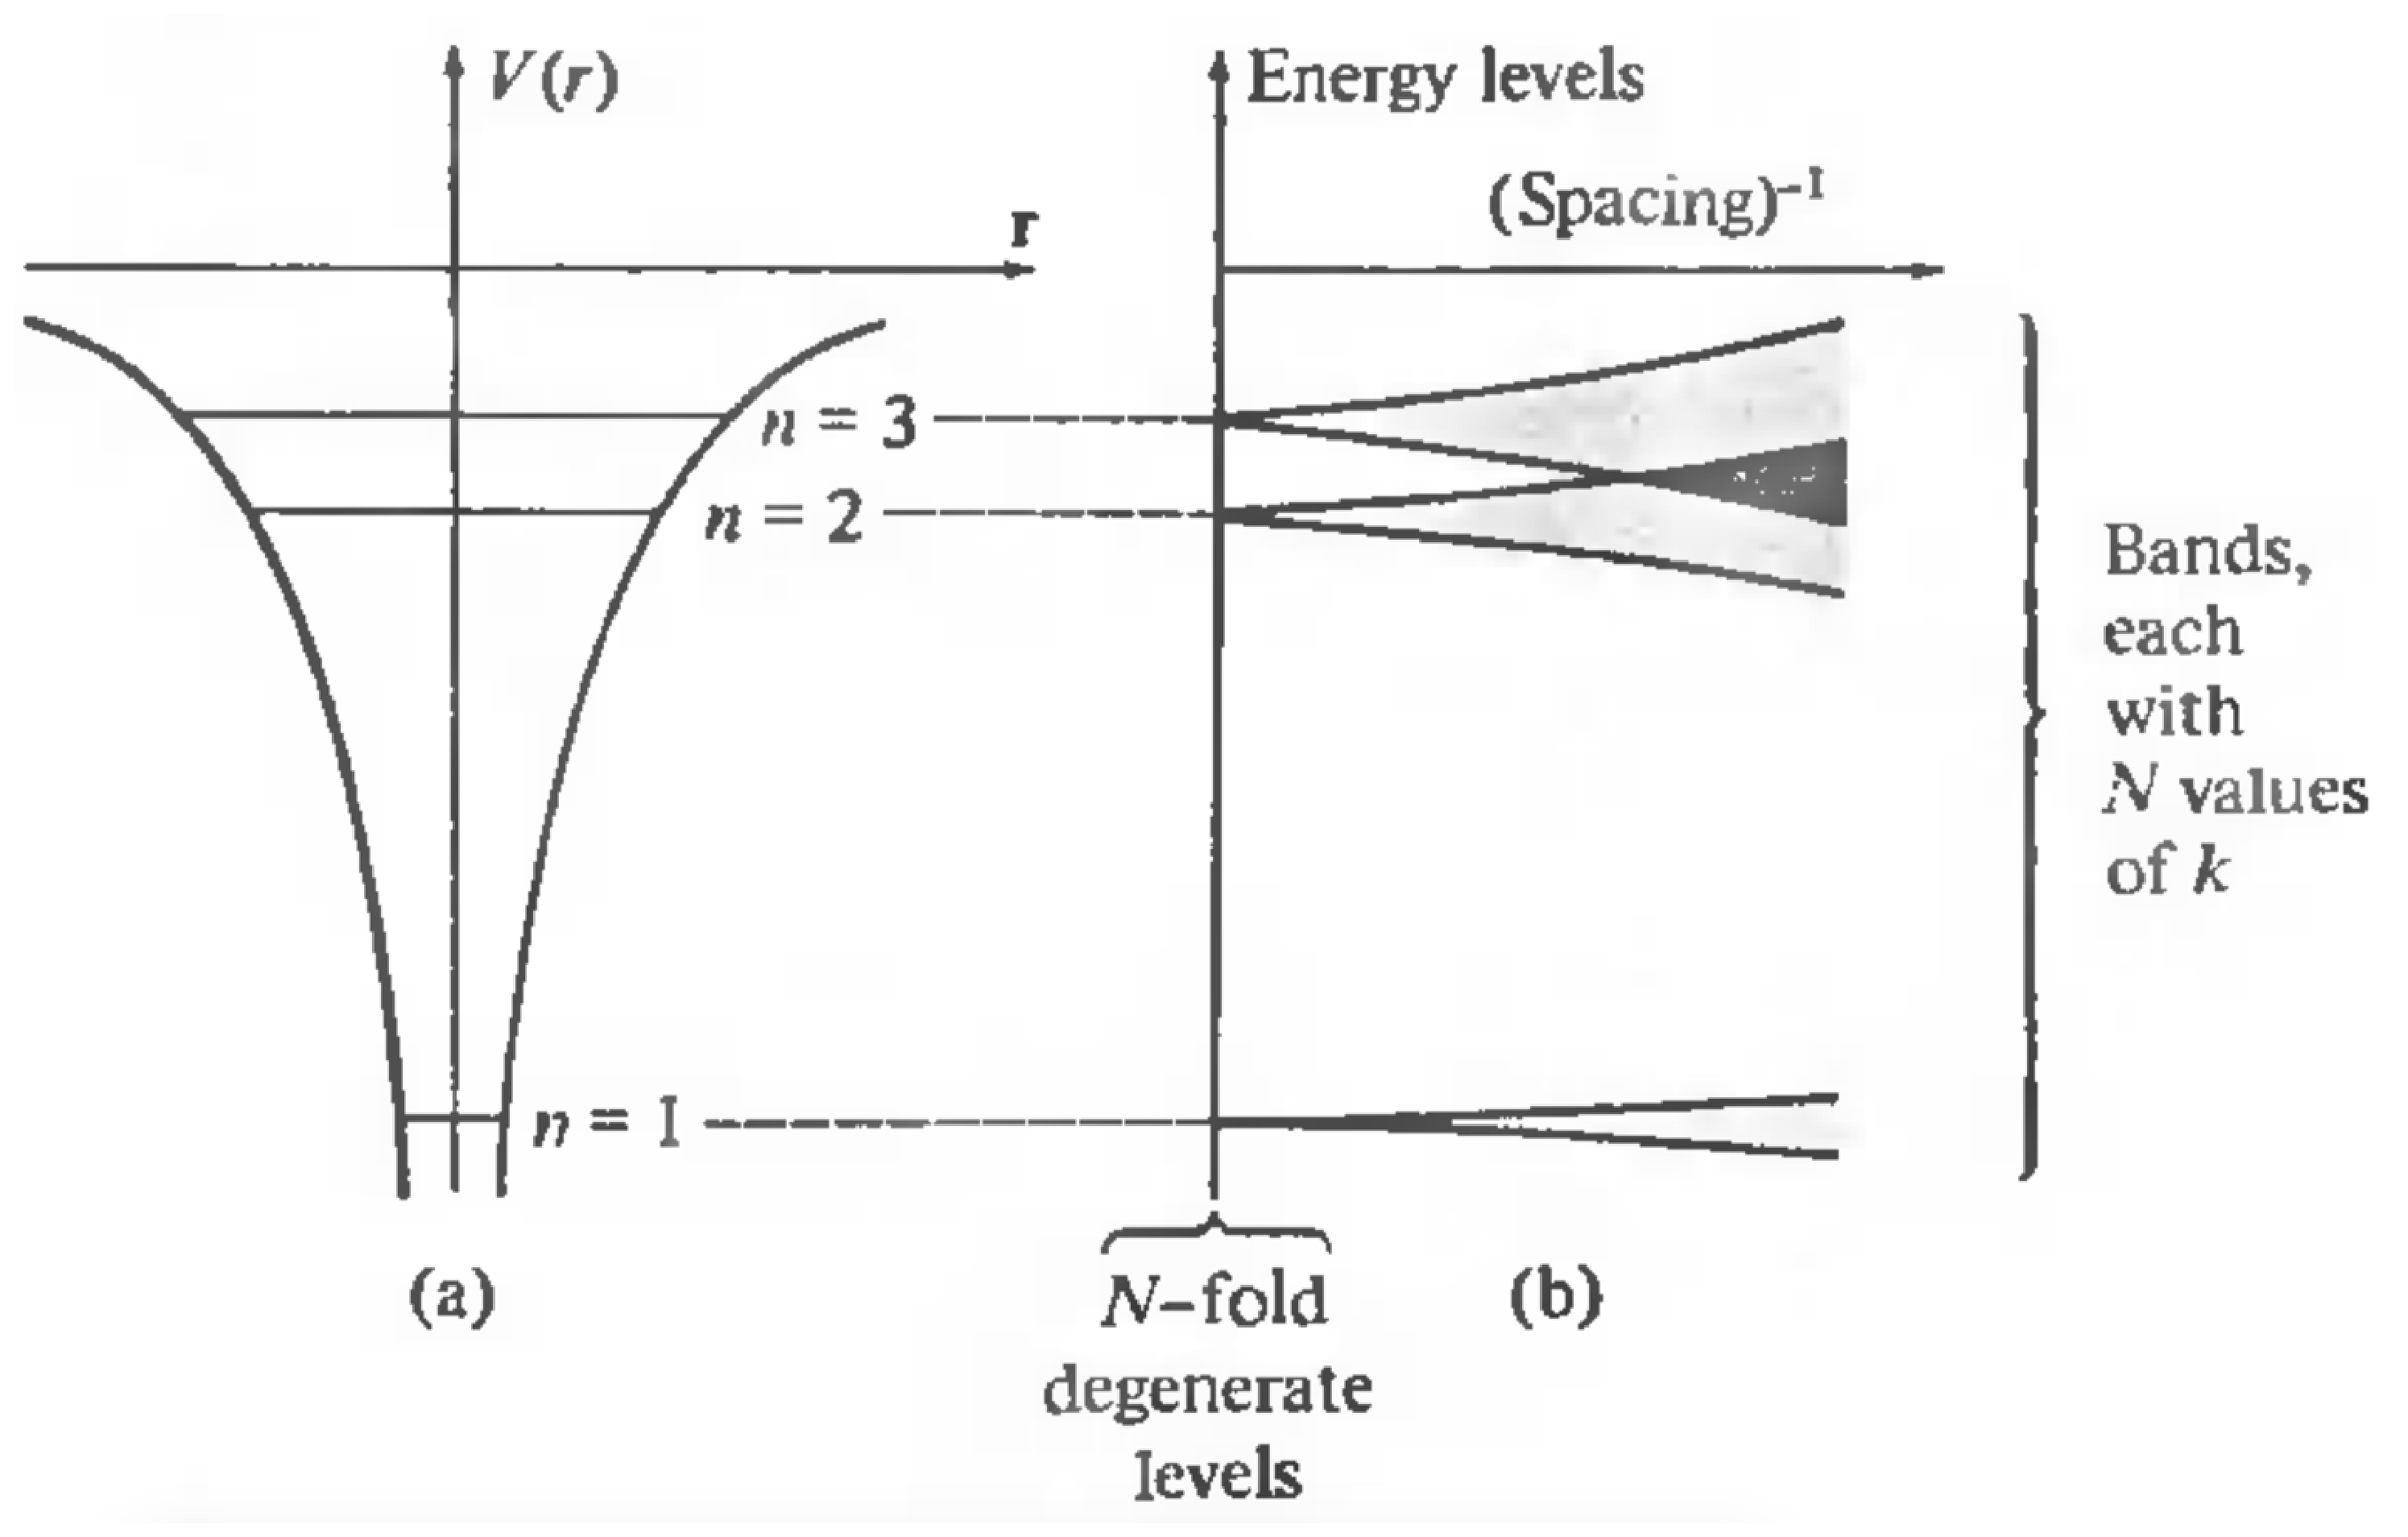
\includegraphics[width=\hsize]{Introduction/band.eps}
  \end{center}
  \caption{原子間距離と電子のエネルギー準位\cite{ashcroft1976}}
  \label{fig:band}
 \end{minipage}
 \begin{minipage}{0.5\hsize}
    \begin{center}
   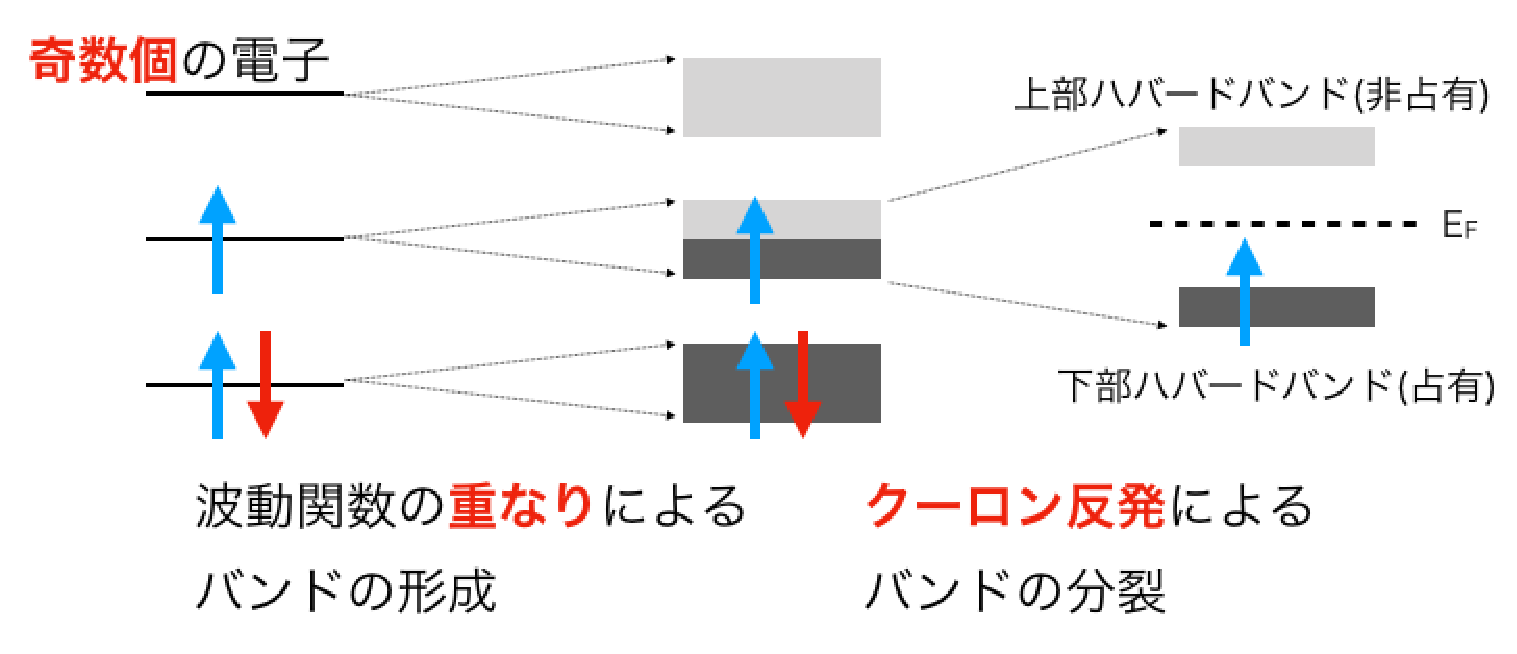
\includegraphics[width=\hsize]{Introduction/Mott_gap.eps}
  \end{center}
  \caption{Mottギャップ}
  \label{fig:Mott_gap}
 \end{minipage}
\end{figure}

Mott絶縁体を元素置換し、キャリアをドープすると超伝導が現れる。図\ref{fig:phase_diagram}に銅酸化物超伝導体の典型的な相図を示す\cite{Andrea2003}。$\rm La_2CuO_4$は反強磁性(AF)のMott絶縁体だが、$\rm Sr$による置換で正孔がドープされ超伝導を示す。ドープ量に対して超伝導転移温度はドーム型の形をしており、あるドープ量で超伝導転移温度は最大となる。$\rm Nd_2CuO_4$も同様に$\rm Ce$による置換で超伝導を示すが、電子がドープされる点が異なる。図に示した二つの相図の特徴は銅酸化物超伝導体に普遍的である\cite{Lee2006}。



\subsection{非平衡過程を用いた超伝導相の制御}
まず非平衡状態における過渡的な超伝導を光を用いて実現した報告に関して述べる。光Faustiらは常伝導相のある銅酸化物に赤外光パルスを入射することで、過渡的な超伝導相が現れることを示した\cite{Fausti,Hunt2015}。図\ref{fig:phase_diagram2}に彼らが用いた$\rm La_{1.8-x}Eu_{0.2}Sr_{x}CuO_4$の相図を示す\cite{Cavalleri2018}。典型的な銅酸化物超伝導体(図\ref{fig:phase_diagram})と同様にドーム状の構造を持ちつつも、$x=1/8$で転移温度に特異的なへこみが見て取れる。この物質はドープ量$x=1/8$となったとき電荷がストライプ状に配列し、超伝導の発現が阻害されることが知られている(ドープ量1/8問題)。彼らはこのストライプ秩序状態の銅酸化物に対して赤外光パルスを印加し格子振動を励起することで、秩序状態を過渡的に破壊し超伝導を実現した。同様にMitranoらはフラーレンとアルカリ金属のインターカレーション$\rm K_3C_{60}$にも過渡的な超伝導相が現れる可能性を示した\cite{Mitrano2016}。これらはパルスを用いて秩序状態を破壊した結果に生じた超伝導であり、元素置換と異なった、非平衡過程を用いたアプローチである。
\begin{figure}[!h]
 \begin{minipage}{0.55\hsize}
    \begin{center}
   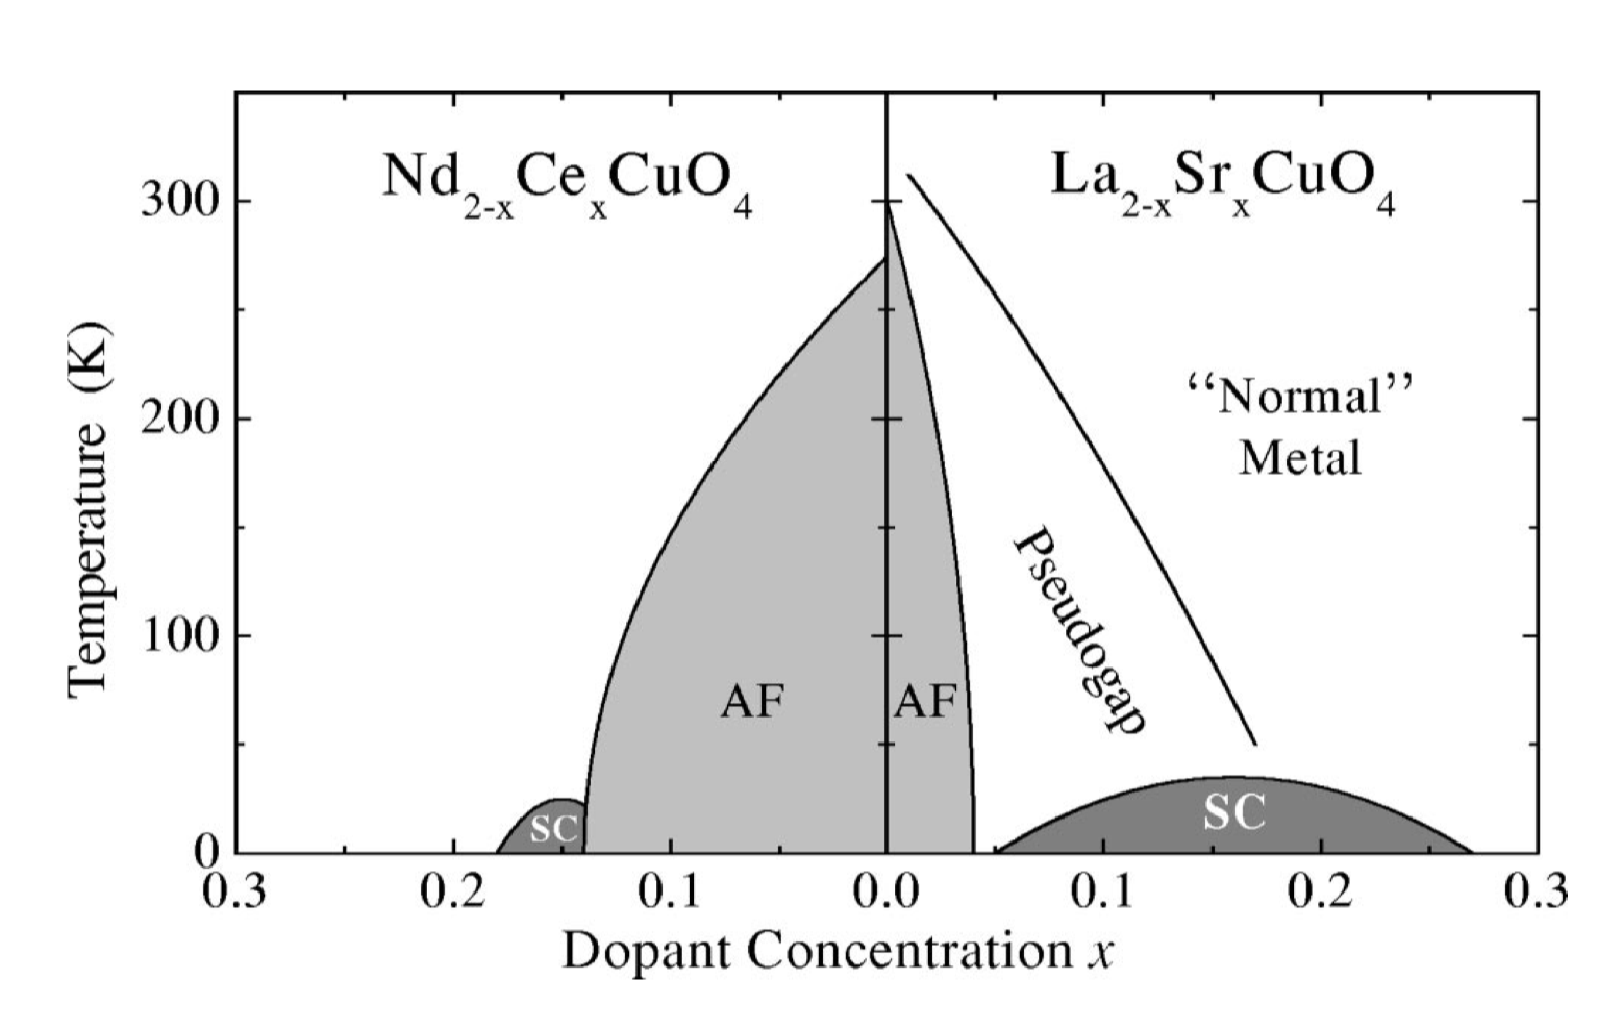
\includegraphics[width=\hsize]{Introduction/phase_diagram.eps}
  \end{center}
  \caption{銅酸化物超伝導体の典型的な相図\cite{Andrea2003}}
  \label{fig:phase_diagram}
 \end{minipage}
 \begin{minipage}{0.45\hsize}
    \begin{center}
   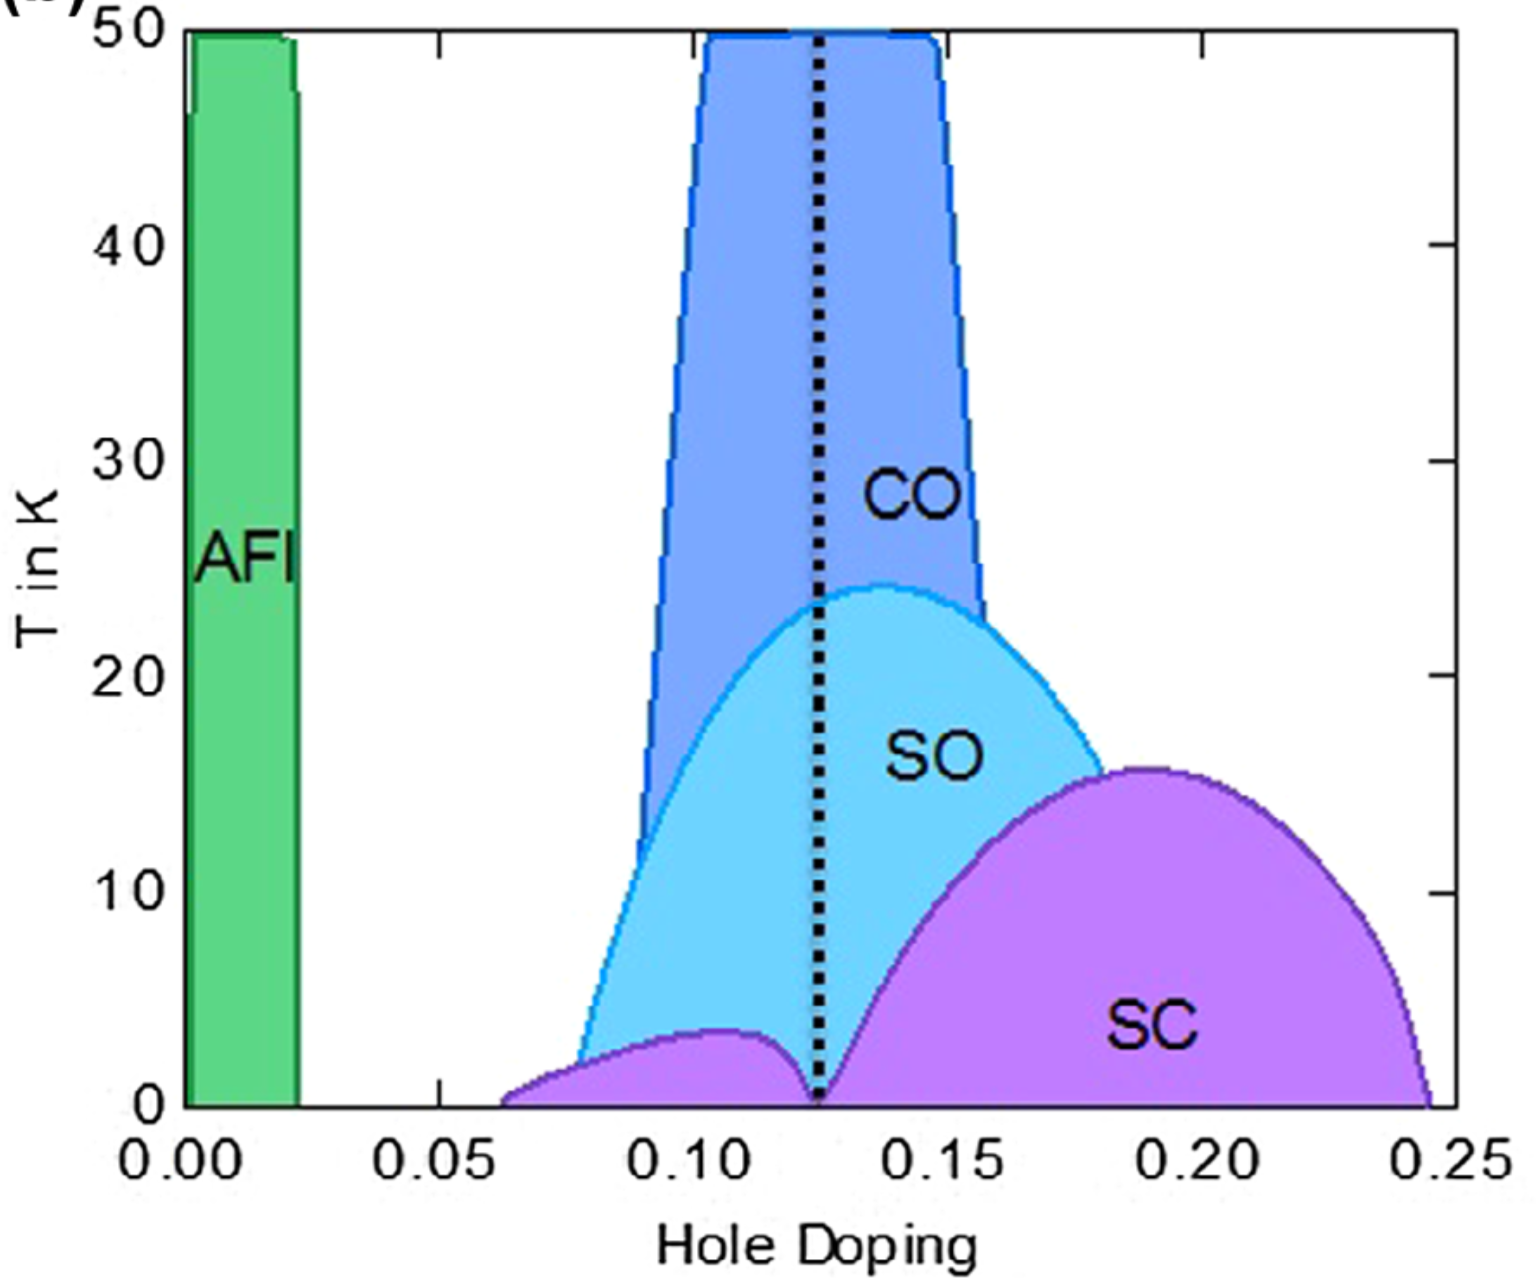
\includegraphics[width=\hsize]{Introduction/phase_diagram2.eps}
  \end{center}
  \caption{銅酸化物超伝導体$\rm La_{1.8-x}Eu_{0.2}Sr_{x}CuO_4$の相図\cite{Cavalleri2018}}
  \label{fig:phase_diagram2}
 \end{minipage}
\end{figure}

つぎに非平衡過程を用いて秩序状態を抑制し、準定常的な超伝導状態を実現した報告に関して述べる。
大池らは電荷が配列し電荷秩序状態となった遷移金属ダイカルコゲナイドIrTe$_2$を電流パルスにより加熱・急冷すると、急冷時に電荷秩序状態の発現が阻害され、競合する超伝導状態が現れることを示した\cite{Oike}。この超伝導状態は準安定であり、数週間以上持続する。さらにパルス強度とパルス幅を適切に調整することで、超伝導から電荷秩序状態を復元できることも示した。これらは急加熱・急冷を用いて競合する秩序状態を抑制した結果に生じた超伝導であり、平衡過程からは到達できない状態(超伝導)を実現できる。
\begin{figure}[!h]
    \begin{center}
   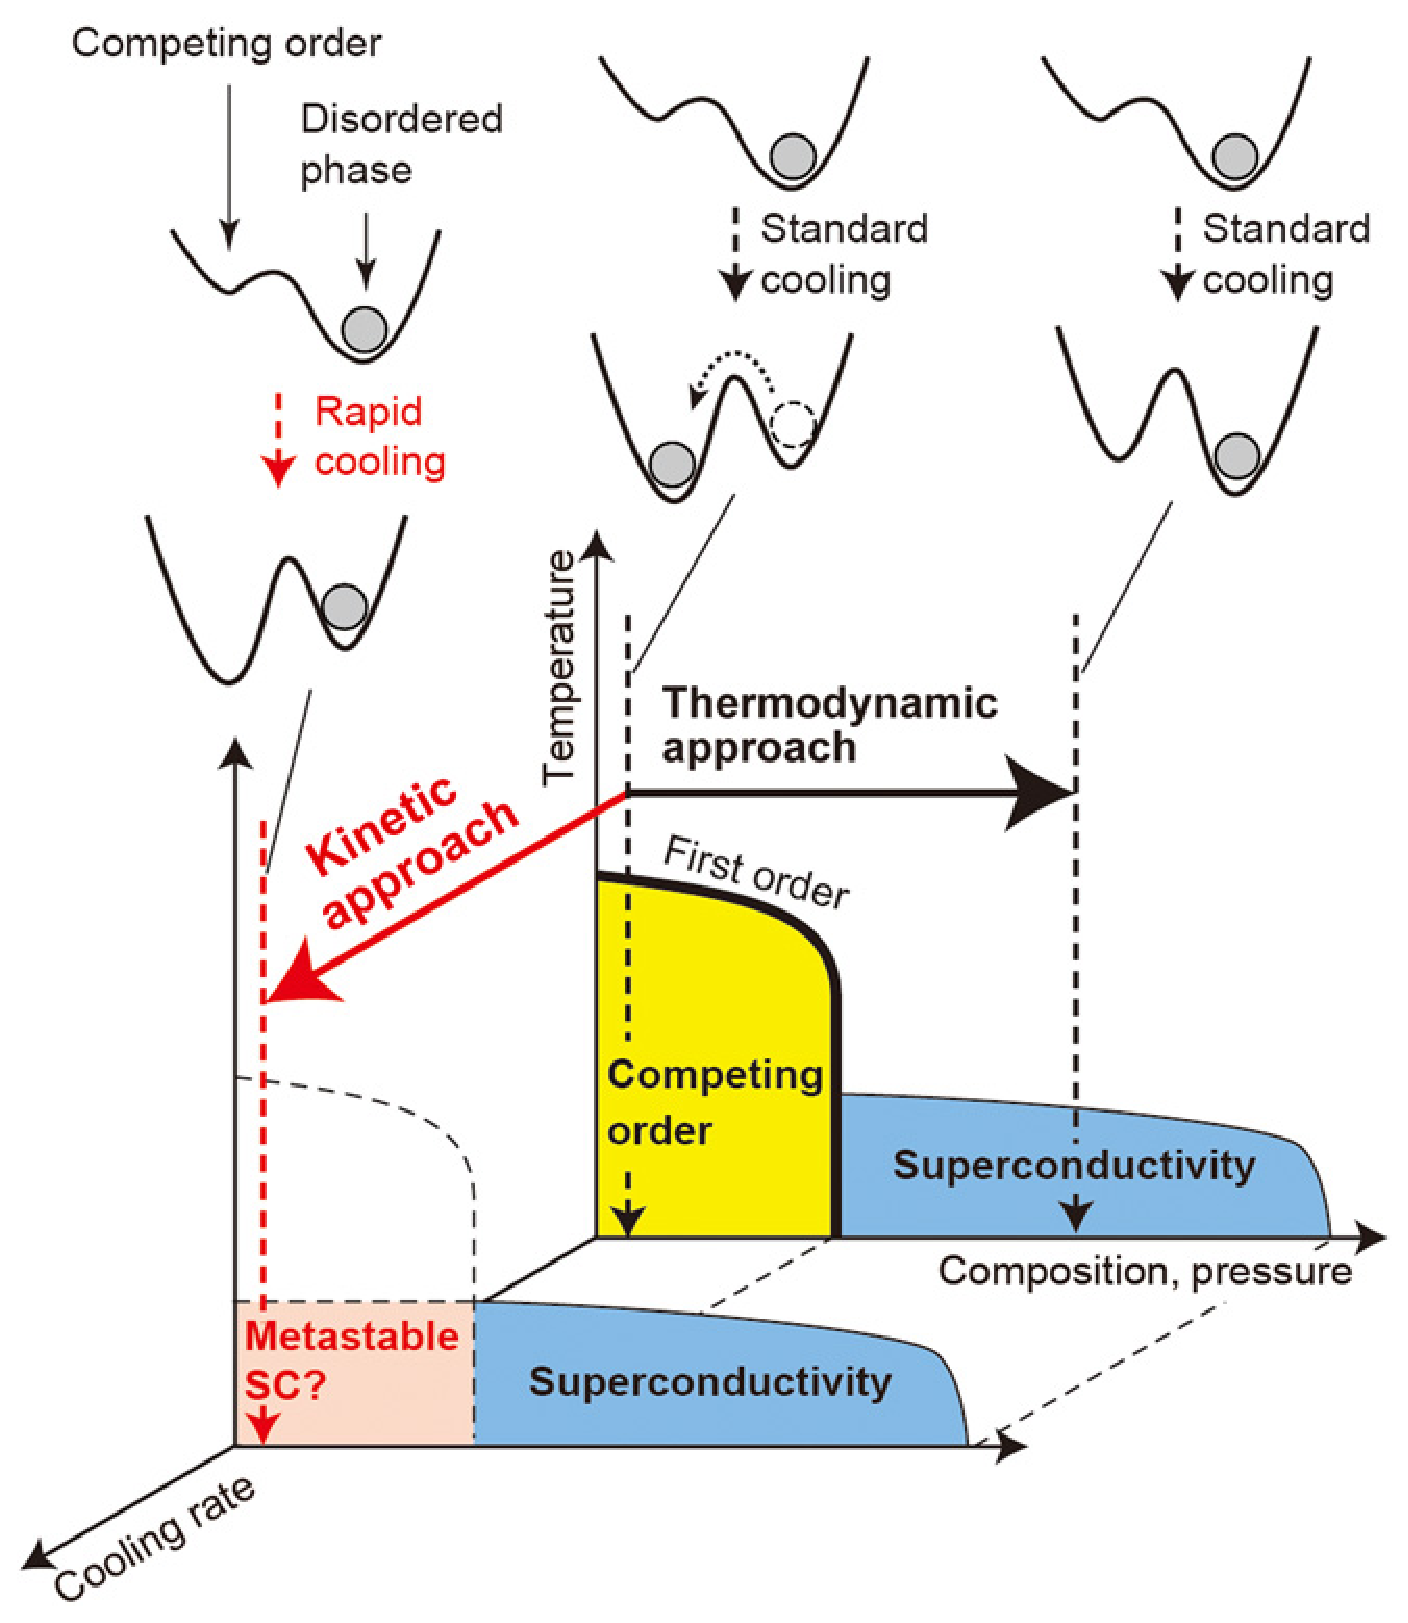
\includegraphics[width=0.6\hsize]{Introduction/kinetic_approach.eps}
  \end{center}
  \caption{}
  \label{fig:phase_diagram2}
\end{figure}


\subsection{スズ}

\subsubsection{物質特性}
スズは286.4Kより高温で正方晶の金属相(βスズ)が安定で、低温で立方晶の半導体相(αスズ)が安定である。図\ref{fig:Sn-Alpha-Beta}にちを示す。


βスズは金属光沢があり、可視域を吸収するαスズに比べ反射率が大きいので、空間的なα相とβ相を測定することができる。図\ref{fig:Sn-Alpha-Beta}にαスズとβスズの見た目の違いを示す\cite{wiki}。
さらに、αスズは立方晶であり、βスズは正方晶である。これらの対称性を比較すると、付録に示すようにとできる。実際このような性質を用いて等方的な相と非等方的な相の対称性の変化を検出できる\cite{Matvienko}。
\begin{figure}[!h]
    \begin{center}
   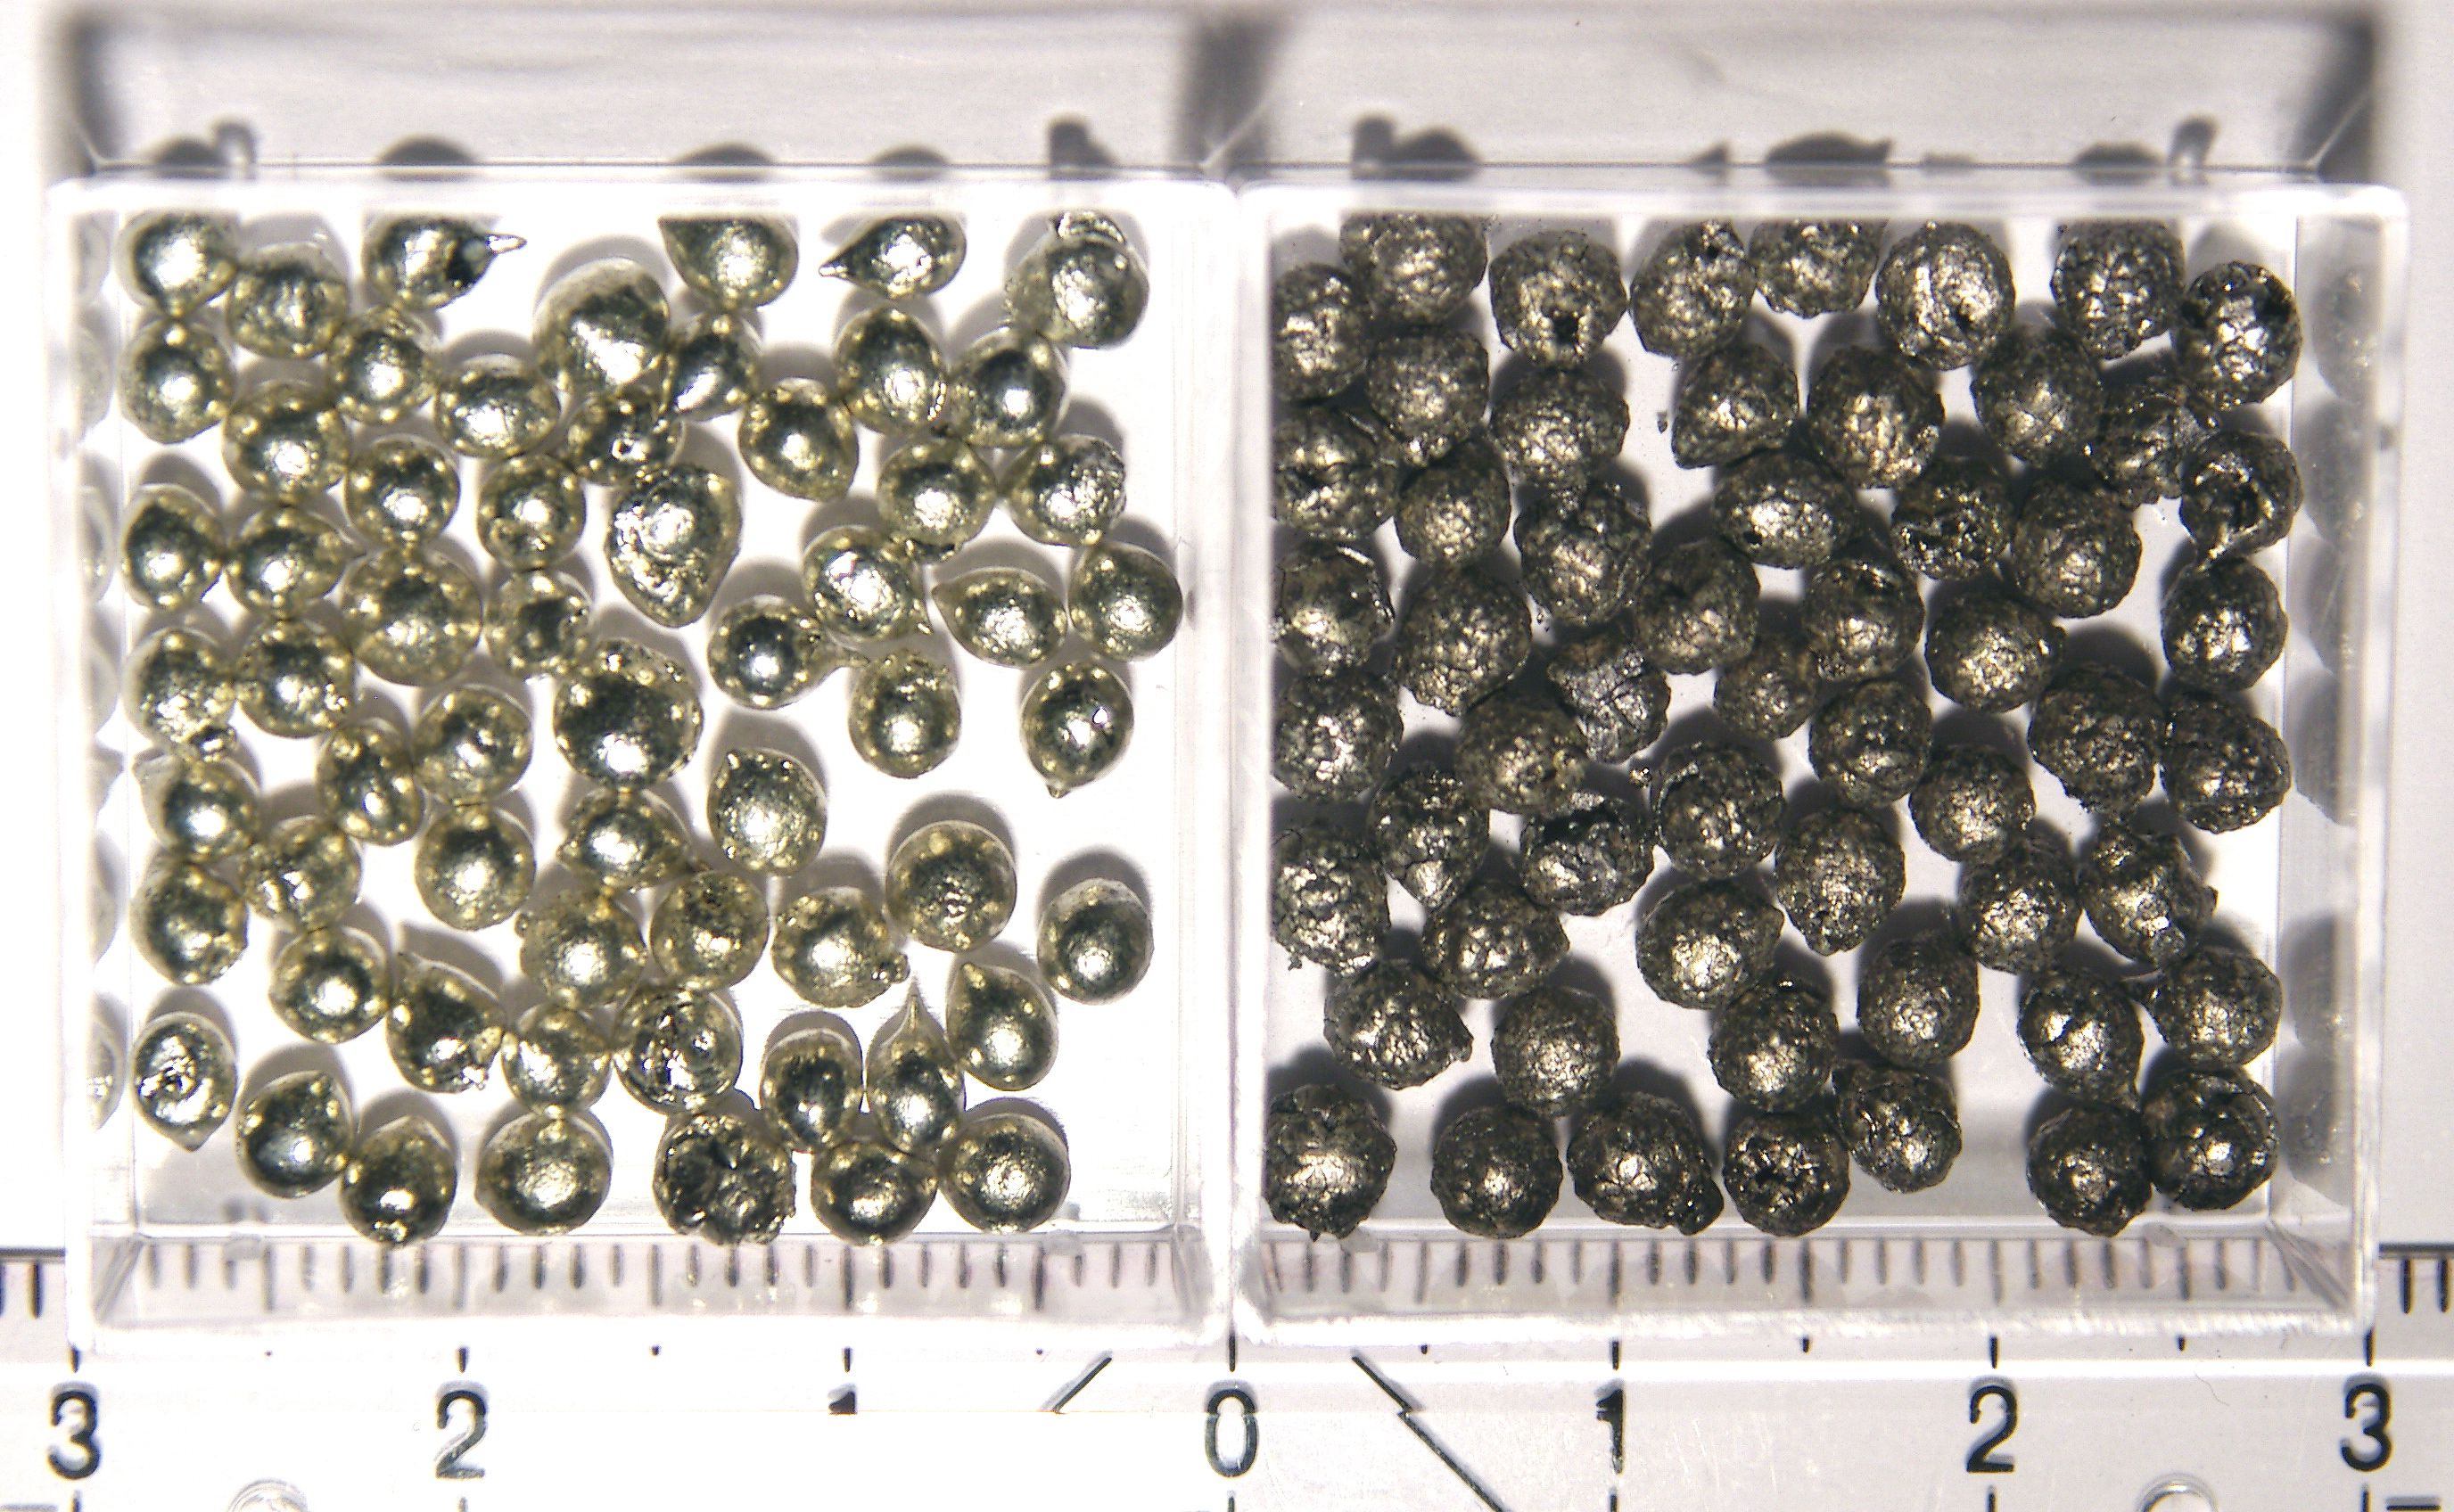
\includegraphics[width=0.9\hsize]{Introduction/Sn-Alpha-Beta.eps}
  \end{center}
  \caption{αスズとβスズの外観 (左: βスズ; 右: αスズ)}
  \label{fig:Sn-Alpha-Beta}
\end{figure}

スズは周期表において14族の元素である。図\ref{fig:group14}に14族の物質構造を示した。Geはスズのひとつ上の周期に属し、金属のPbはひとつ下の周期に属する。SiとGe、半導体のスズはダイアモンド構造をとる。金属のスズはPbと同様に金属的な高い導電性を示す。室温付近で金属と半導体のエネルギー差は小さく、どちらも安定に存在する。図\ref{fig:bandgaps}に14族半導体のバンドギャップ$\epsilon_g$と最近接原子間距離$R_{nn}$を示す\cite{Yonezawa}。最近接原子間距離$R_{nn}$が大きいほどバンドギャップは小さくなり、半導体スズはバンドが閉じるギリギリのところにあることが見て取れる。半導体スズのバンドギャップは0.08eVと非常に小さい。温度を上げると半導体スズの$R_{nn}$はさらに大きくなり、バンドが閉じ金属的になる。この半導体-金属転移はブロッホ・ウィルソン転移(タイプ2)と呼ばれる\cite{Yonezawa}。

\begin{figure}[!h]
 \begin{minipage}{0.4\hsize}
  \begin{center}
   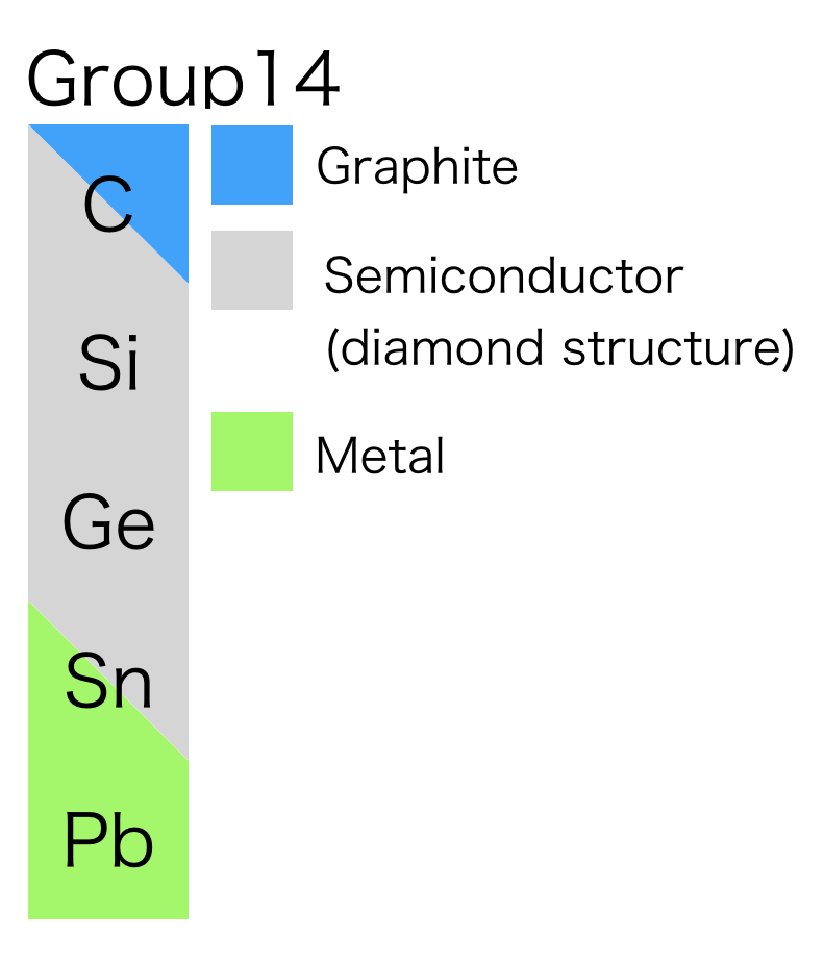
\includegraphics[width=50mm]{Introduction/group14.eps}
  \end{center}
  \caption{14族元素の相}
  \label{fig:group14}
 \end{minipage}
 \begin{minipage}{0.6\hsize}
  \begin{center}
   
\includegraphics[width=90mm]{Introduction/bandgaps.eps}
  \end{center}
  \caption{14族半導体のバンドギャップ$\epsilon_g$と最近接原子間距離$R_{nn}$\cite{Yonezawa}}
  \label{fig:bandgaps}
 \end{minipage}
\end{figure}


\subsubsection{相転移}
核生成と相転移の進行

半導体相は$\rm \alpha$相と呼ばれダイアモンド構造を持つ。
αスズとβスズの構造転移には27\%程度の大きな体積変化が伴う。したがって、核生成は試料の内部より表面から始まりやすい\cite{Cornelius}。

モル体積を比較すると27\%程度異なるため、

図\ref{fig:alpha-to-beta}と図\ref{fig:beta-to-alpha}にそれぞれ、αスズからβスズへの転移にかかる時間と、βスズからαスズへの転移にかかる時間を示す\cite{Nogita}。
図\ref{fig:alpha-to-beta}から、αスズからβスズへの転移は温度が転移温度よりも十分に高ければ3分未満で進行する。一方、図\ref{fig:beta-to-alpha}から、
最速でもβスズからαスズへの転移は、それ以上の時間がかかる可能性が示唆される。
αスズとβスズは室温で安定である。
\begin{figure}[!h]
 \begin{minipage}{0.5\hsize}
  \begin{center}
   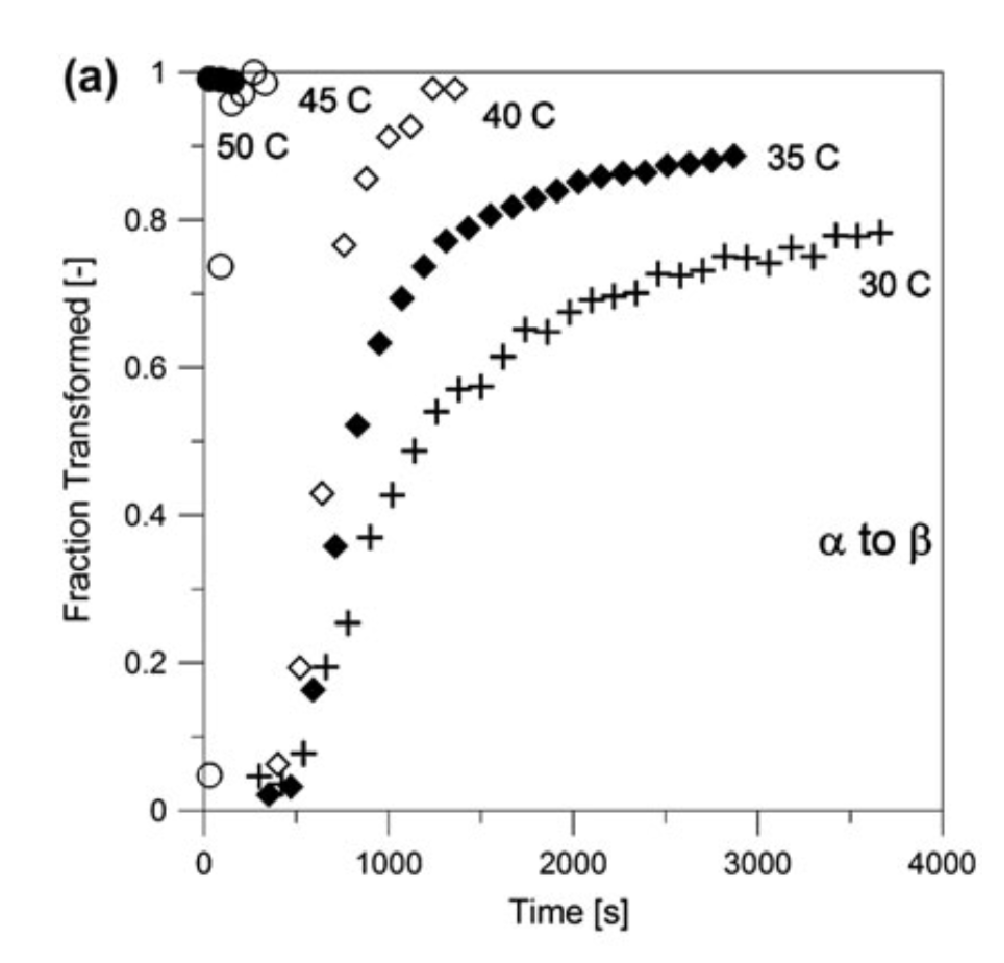
\includegraphics[width=\hsize]{Introduction/alpha-to-beta.eps}
  \end{center}
  \caption{αスズからβスズへの転移にかかる時間}
  \label{fig:alpha-to-beta}
 \end{minipage}
 \begin{minipage}{0.5\hsize}
    \begin{center}
   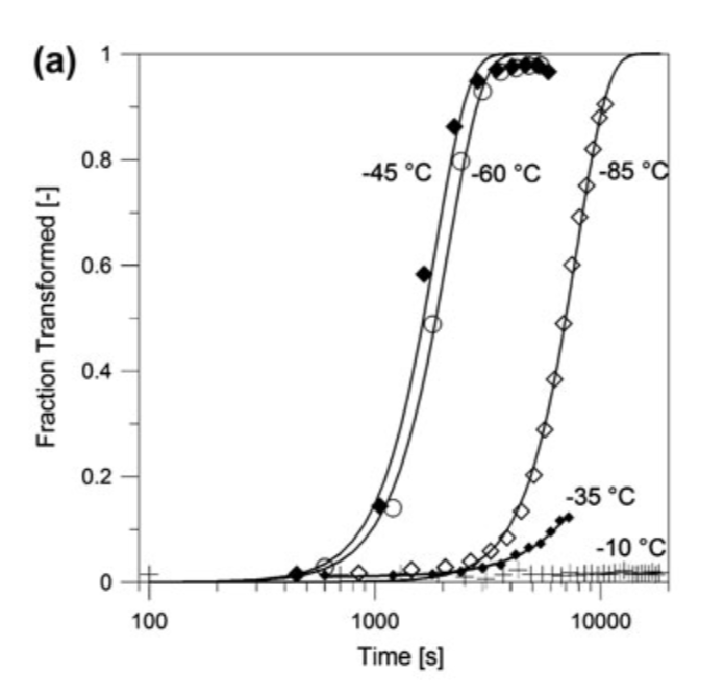
\includegraphics[width=\hsize]{Introduction/beta-to-alpha.eps}
  \end{center}
  \caption{βスズからαスズへの転移にかかる時間}
  \label{fig:beta-to-alpha}
 \end{minipage}
\end{figure}

\begin{figure}[!h]
    \begin{center}
   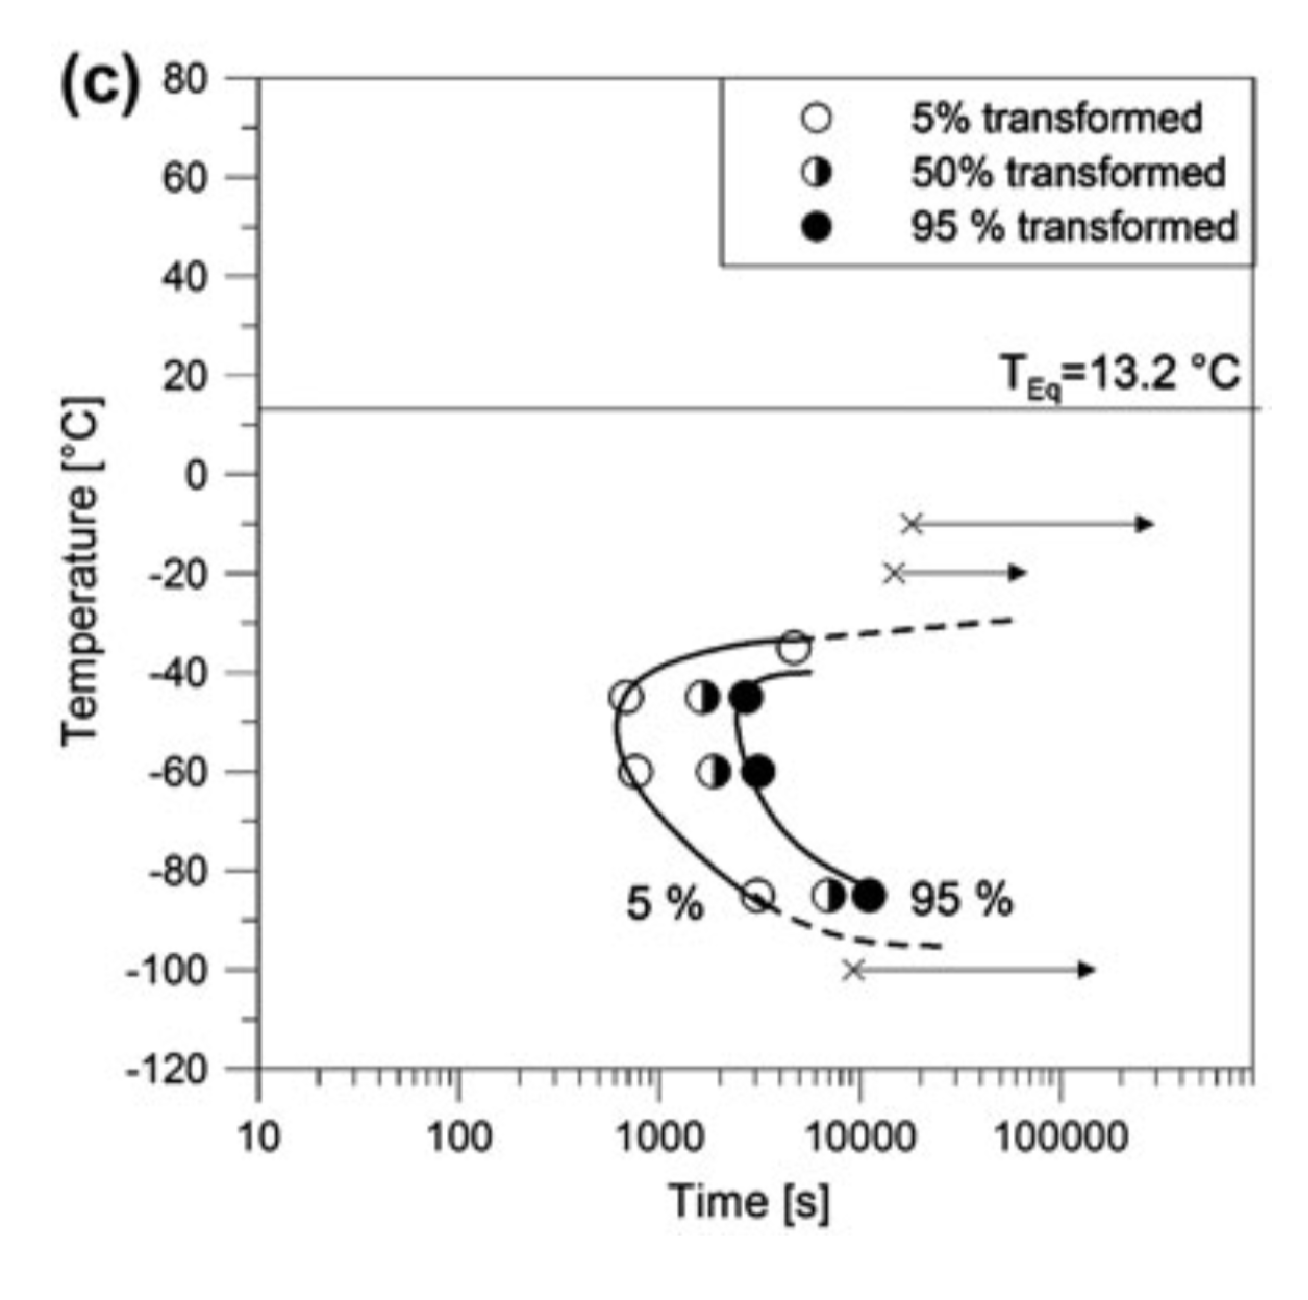
\includegraphics[width=130mm]{Introduction/TTT.eps}
  \end{center}
  \caption{温度と$\beta-\alpha$転移時間の関係(TTT)\cite{Nogita}}
  \label{fig:TTT}
\end{figure}

αスズは半導体(バンドギャップエネルギー$\rm E_G=0.018eV$)であり低温になればなるほど抵抗が大きい。一方、βスズは金属であり低温になればなるほど抵抗が小さくなる。また室温付近でαスズとβスズの抵抗を比較してもβスズの方が2桁程度小さい。\cite{} したがって、抵抗測定を行うと相転移が起こったかどうかもわかる。



\subsection{スズ-Geコンポジット試料の特性}
図\ref{fig:GeSn_phase}にGe-Snコンポジット(合金)の相図を示す\cite{Olesinski1984}。共晶型の相図であり、スズ-Ge共晶点に置けるGe固溶の限界は0.3\%程度と言われている\cite{Thurmond1960}。
\begin{figure}[!h]
 \begin{minipage}{\hsize}
    \begin{center}
   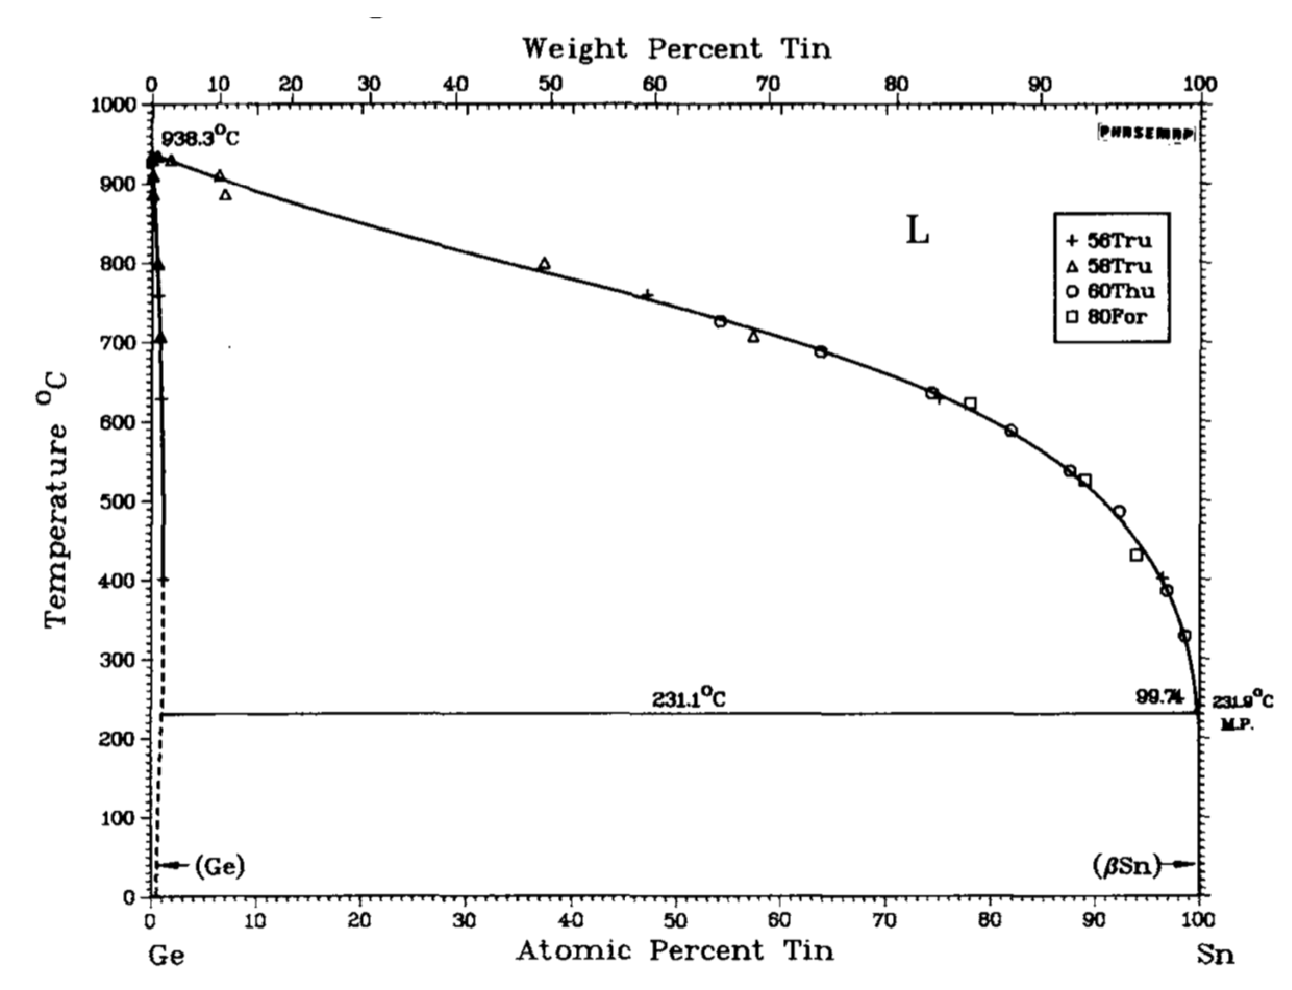
\includegraphics[width=0.8\hsize]{Introduction/GeSn_phase.eps}
  \end{center}
  \caption{Ge-Sn合金の相図\cite{Olesinski1984}}
  \label{fig:GeSn_phase}
 \end{minipage}
 \begin{minipage}{\hsize}
    \begin{center}
   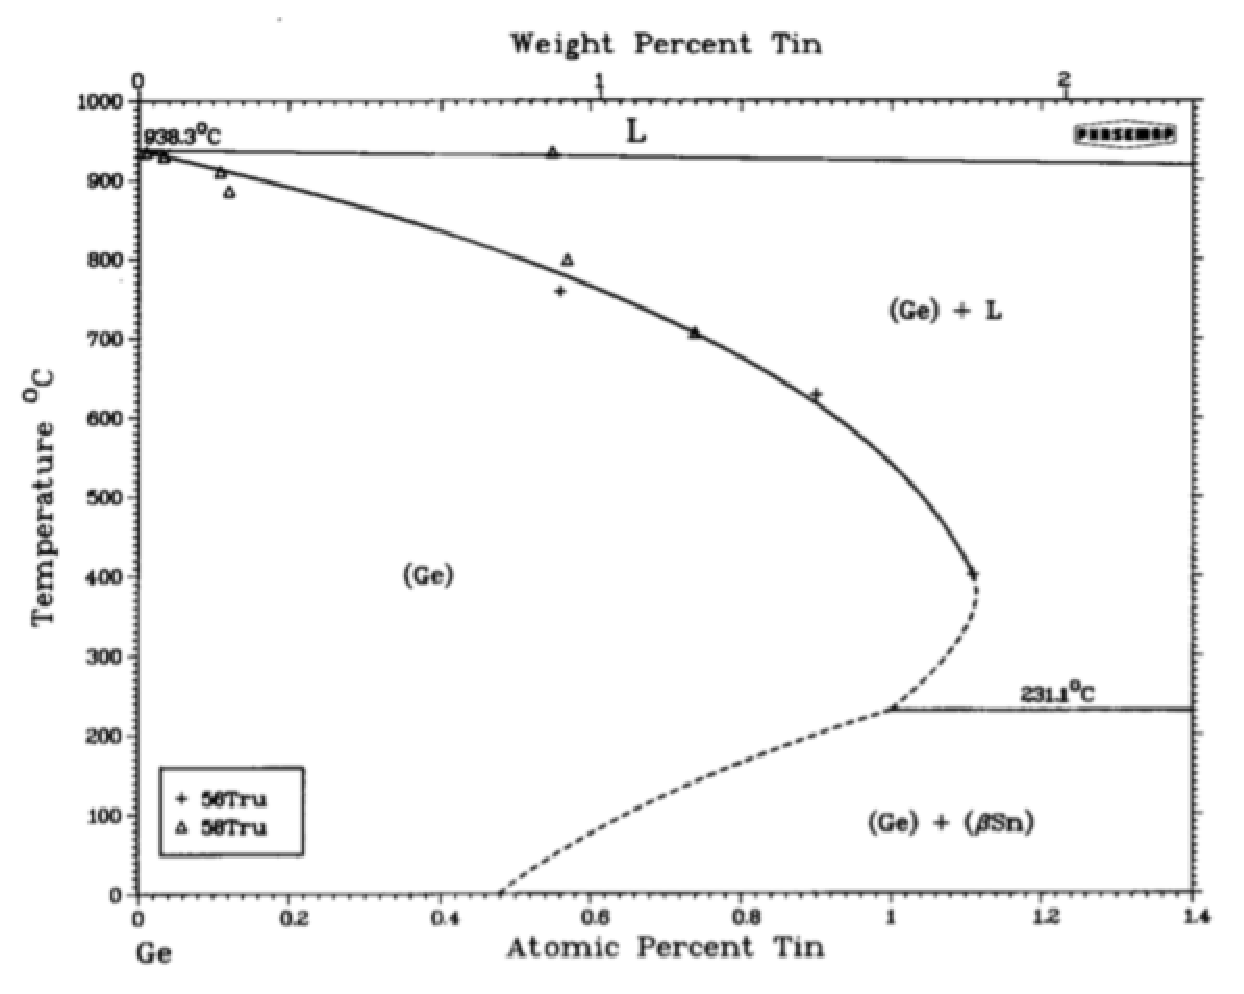
\includegraphics[width=0.8\hsize]{Introduction/GeSn_phase2.eps}
  \end{center}
  \caption{Ge-Sn合金の相図(Geリッチ領域を拡大したもの)\cite{Olesinski1984}}
  \label{fig:GeSn_phase2}
   \end{minipage}
\end{figure}

SiとGeと半導体スズはすべて同一のダイアモンド構造をとることから、半導体スズにSiやGeを少量添加すると安定化することが示唆されている\cite{Ewald1954,Gallerneault1983}。

図\ref{fig:Ge_Stabilized_Sn}にGe添加量と半導体-金属転移温度の関係を示した\cite{Vnuk1984}。Ge添加量を1\%程度まで増やすと転移温度が大きくなることが見て取れる。
\begin{figure}[!h]
    \begin{center}
   \includegraphics[width=0.7\hsize]{Introduction/Ge_Stabilized_Sn.eps}
  \end{center}
  \caption{Ge添加量とスズの$\alpha-\beta$転移温度\cite{Vnuk1984}}
  \label{fig:Ge_Stabilized_Sn}
\end{figure}

一方、Matvienkoらの研究\cite{Matvienko}によると、β相からα相への変換はα-β相界面でのβ相の塑性変形が重要な役割を果たしており、Geを添加するとβ相中の欠陥の拡散が遅くなりα-β変換が阻害される。その結果、図\ref{fig:Ge_content}に示したように、Ge添加量とα-β相界面の移動速度の関係を示した\cite{Matvienko}。Ge添加量が0 at. \%から0.3 at. \%(2 wt. \%)程度までは、添加量を多くすると転移速度が遅くなってゆくことが見て取れる。
%0.3mol\%= 0.003*32/(0.997*50+0.003*32)質量\%
\begin{figure}[!h]
    \begin{center}
   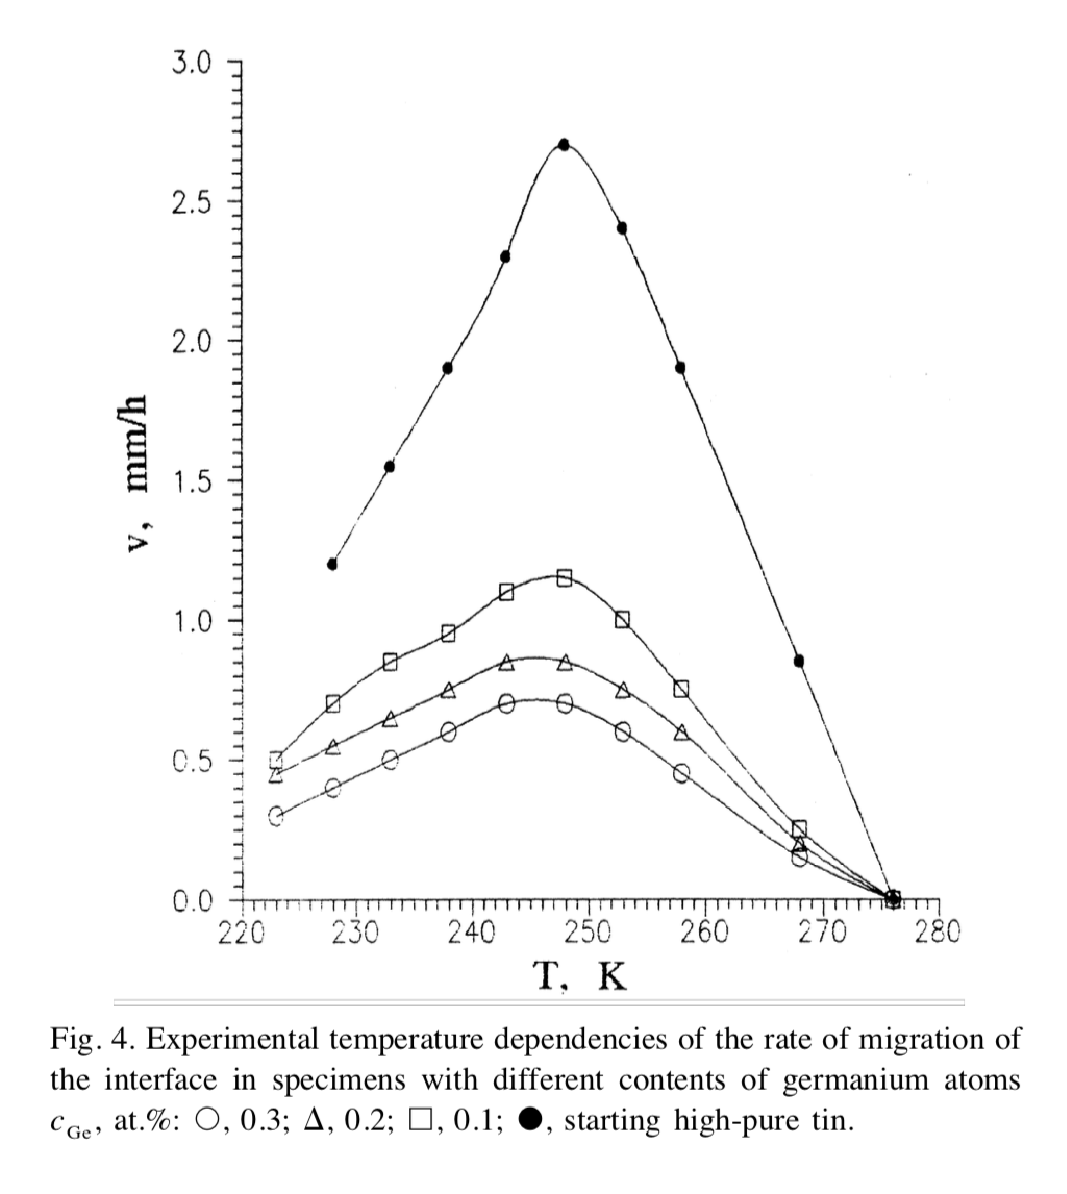
\includegraphics[width=0.9\hsize]{Introduction/Ge_content.eps}
  \end{center}
  \caption{Ge添加量と$\beta-\alpha$転移速度の関係\cite{Matvienko}}
  \label{fig:Ge_content}
\end{figure}

\clearpage
